\chapter{基于用户交互的模型改善}
通过自动化算法生成的模型难免含有算法设计者的主观想法在其中,比如树木何时应该分支,何时
应该合并等等。并且算法在处理实际的模型时,通常带有一定的二义性。未免过于主观地决定了模
型的最终成型,本文提倡在自动化生成模型以后,应该将模型
的建立延迟到应用程序,或者使用该模型的最终用户。这样可以使得本文所建立的一系列方法适用于
更广的情形。将自动化算法与人工交互联合使用,可以大大地提高最终模型与具体需求之间的耦合度。

本文根据此需求,开发完成了一个树木模型用户交互平台,可以用于对本文的基于图像所建立的树木
模型进行进一步地编辑和完善。该平台集成了几种不同轻量化级别的模型表示,模型的编辑,算法的
演示等功能,大大的提高了算法验证的直观度和用户与应用级模型改善的方便性。该平台的具体功能
见用例图\ref{fig:usecase}。

\begin{figure}[H]
	\centering
	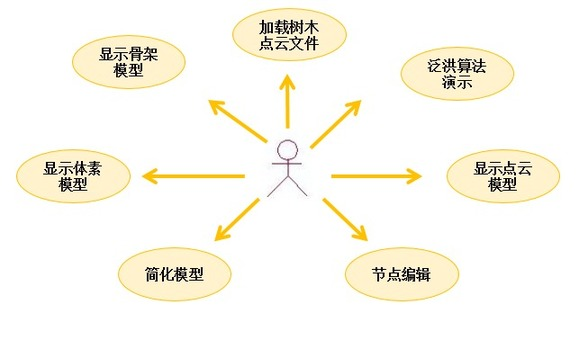
\includegraphics[height=6cm]{usecase.jpg}
	\caption{用户交互平台用例图}
	\label{fig:usecase}
\end{figure}

对于每个用例,本文用表格和图片对其进行进一步说明,由于本文并不将重点放在软件开发上,所以
在本文中未给出具体的系统分析和设计。本文试图对该用户交互平台的功能进行阐述,从而在功能性上
对自动化算法进行人工加强和改善。

\clearpage
\section{加载树木点云文件}

\begin{figure}[H]
	\centering
	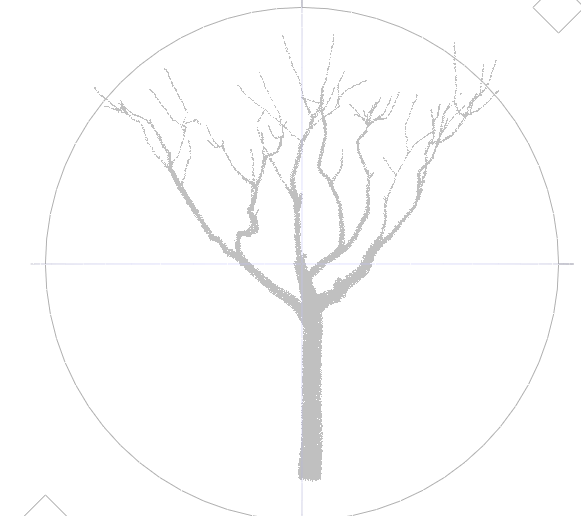
\includegraphics[height=6cm]{uc1.png}
	\caption{用例1图示:用开源软件MeshLab打开的树木点云文件}
	\label{fig:uc1}
\end{figure}

\begin{table}[H]
	\centering
\begin{tabular}{|l|p{8cm}|}
	\hline
	用例名称: & 加载树木点云文件\\
	\hline
	用例标志号: & 1\\
	\hline
	参与者: & 用户\\
	\hline
	简要说明: & 用户可以按键'l'来加载存储为".ply"开源格式的名为"Tree.ply"的点云文件,该
	后缀名的点云模型可以用开源软件Meshlab来打开观察,如图\ref{fig:uc1}\\
	\hline
	前置条件: & 树木的模型文件存在于./Models/文件夹下\\
	\hline
	基本事件流: & 1. 用户按下'l'键\\
	 & 2. 系统去./Models/文件夹下搜索名为"Tree.ply"的点云文件\\
	 & 3. 将点云文件加载入内存\\
	 & 4. 用例终止\\
	\hline
	异常事件流: & 1. 若点云文件不存在,则不会加载入内存\\
	\hline
	后置条件: & 无\\
	\hline
\end{tabular}
\end{table}

\clearpage
\section{显示骨架模型}
\begin{figure}[H]
	\centering
	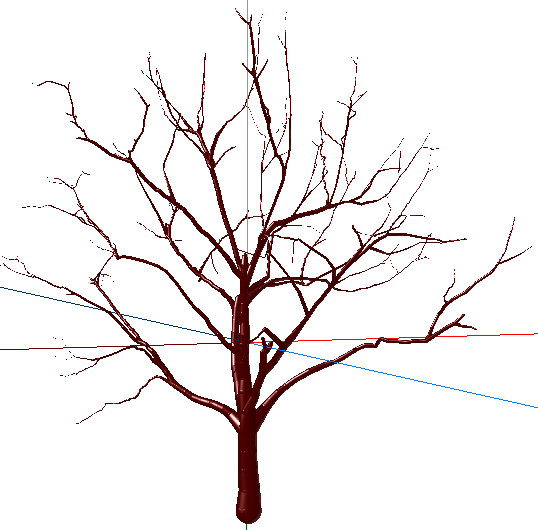
\includegraphics[height=6cm]{uc2.png}
	\caption{用例图示:显示骨架模型}
	\label{fig:uc2}
\end{figure}

\begin{table}[H]
	\centering
\begin{tabular}{|l|p{8cm}|}
	\hline
	用例名称: & 显示骨架模型\\
	\hline
	用例标志号: & 2\\
	\hline
	参与者: & 用户\\
	\hline
	简要说明: & 用户可以通过选择显示骨架模型来观察树木的骨架,具体效果见图\ref{fig:uc2}\\
	\hline
	前置条件: & 树木的模型文件已经被加载进入软件平台\\
	\hline
	基本事件流: & 1. 用户按下'm'键将显示模式切换到骨架模式\\
	 & 2. 将树木骨架模型用冯氏光照模型渲染至视口\\
	 & 3. 用例终止\\
	\hline
	异常事件流: & 1. 若模型文件未加载,则不会显示对应模型骨架\\
	\hline
	后置条件: & 无\\
	\hline
\end{tabular}
\end{table}

\clearpage
\section{显示点云模型}
\begin{figure}[H]
	\centering
	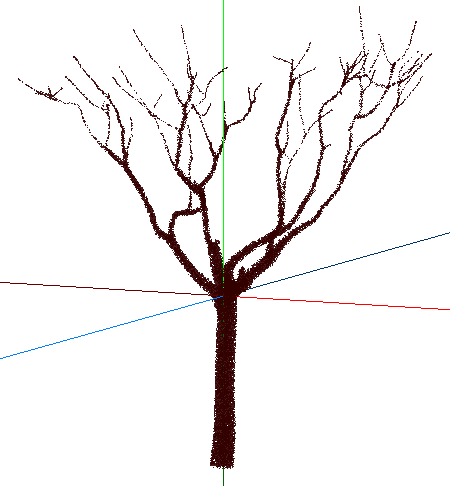
\includegraphics[height=6cm]{uc3.png}
	\caption{用例图示:显示点云模型}
	\label{fig:uc3}
\end{figure}

\begin{table}[H]
	\centering
\begin{tabular}{|l|p{8cm}|}
	\hline
	用例名称: & 显示点云模型\\
	\hline
	用例标志号: & 3\\
	\hline
	参与者: & 用户\\
	\hline
	简要说明: & 用户可以通过选择显示点云模型来观察树木的点云表示,具体效果见图\ref{fig:uc3}\\
	\hline
	前置条件: & 树木的模型文件已经被加载进入软件平台\\
	\hline
	基本事件流: & 1. 用户按下'm'键切换显示模式到点云模式\\
	 & 2. 将点云模型用平滑光照模型渲染至视口\\
	 & 3. 用例终止\\
	\hline
	异常事件流: & 1. 若模型文件未加载,则不会显示对应点云模型\\
	\hline
	后置条件: & 无\\
	\hline
\end{tabular}
\end{table}

\clearpage
\section{显示体素模型}
\begin{figure}[H]
	\centering
	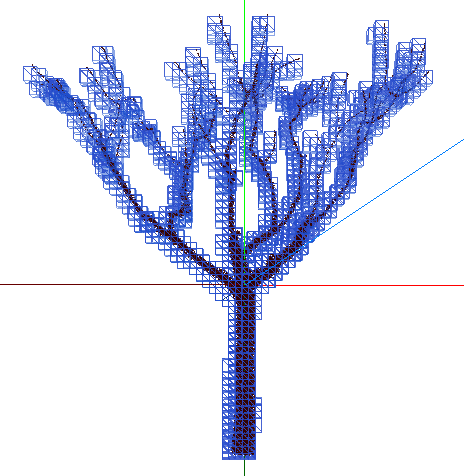
\includegraphics[height=6cm]{uc4.png}
	\caption{用例图示:显示体素模型}
	\label{fig:uc4}
\end{figure}

\begin{table}[H]
	\centering
\begin{tabular}{|l|p{8cm}|}
	\hline
	用例名称: & 显示体素模型\\
	\hline
	用例标志号: & 4\\
	\hline
	参与者: & 用户\\
	\hline
	简要说明: & 用户可以通过选择显示体素模型来观察树木的体素表示,具体效果见图\ref{fig:uc4}\\
	\hline
	前置条件: & 树木的模型已经被加载进入软件平台\\
	\hline
	基本事件流: & 1. 用户按下'v'键\\
	 & 2. 将体素模型用冯氏光照模型渲染至视口\\
	 & 3. 用例终止\\
	\hline
	异常事件流: & 1. 若模型文件不存在,则不会显示对应点云模型\\
	\hline
	后置条件: & 无\\
	\hline
\end{tabular}
\end{table}

\clearpage
\section{节点编辑}
\begin{figure}[H]
	\centering
	\subfloat[节点插入(前)]{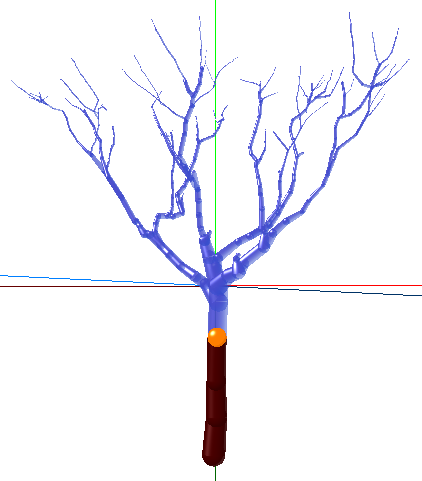
\includegraphics[height=4cm]{uc5_ins1.png}}\hspace{3em}
	\subfloat[节点删除(前)]{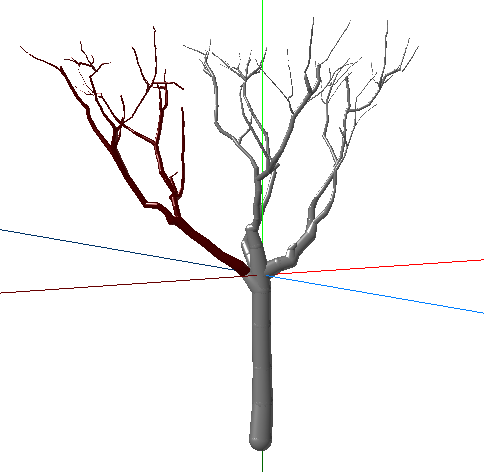
\includegraphics[height=4cm]{uc5_rm1.png}}\hspace{3em}
	\subfloat[节点移动(前)]{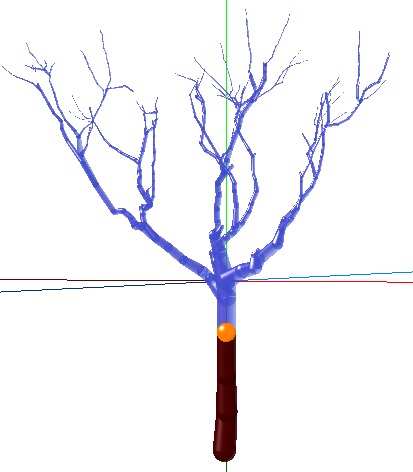
\includegraphics[height=4cm]{uc5_mv1.png}}\hspace{3em}
	\subfloat[节点插入(后)]{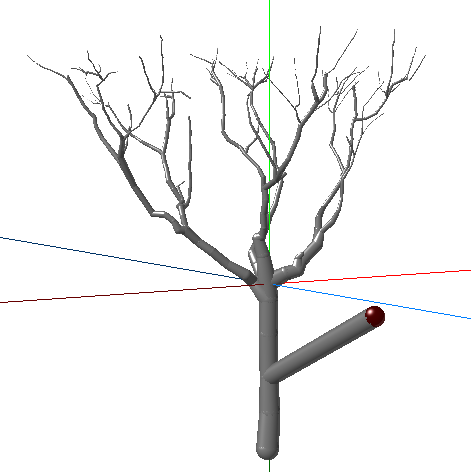
\includegraphics[height=4cm]{uc5_ins2.png}}\hspace{3em}
	\subfloat[节点删除(后)]{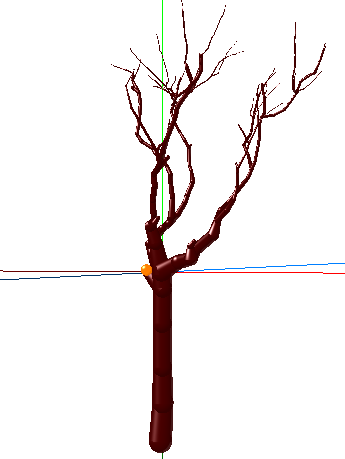
\includegraphics[height=4cm]{uc5_rm2.png}}\hspace{3em}
	\subfloat[节点移动(后)]{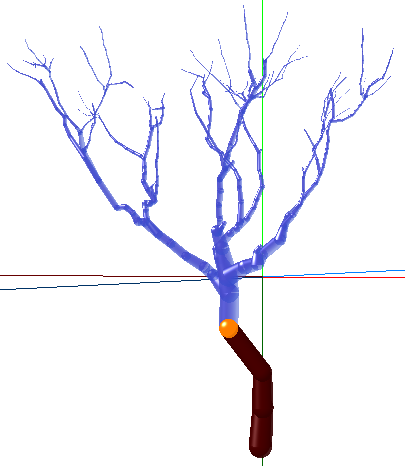
\includegraphics[height=4cm]{uc5_mv2.png}}\hspace{3em}
	\caption{用例图示:节点编辑}
	\label{fig:uc5}
\end{figure}

\begin{table}[H]
	\centering
\begin{tabular}{|l|p{8cm}|}
	\hline
	用例名称: & 节点编辑\\
	\hline
	用例标志号: & 5\\
	\hline
	参与者: & 用户\\
	\hline
	简要说明: & 用户可以通过选中特定的节点,对其进行丰富的编辑操作,具体效果见图\ref{fig:uc5}\\
	\hline
	前置条件: & 树木的显示模式为骨架模型\\
	\hline
	基本事件流: & 1. 用户按下'g'键\\
	 & 2. 树木骨架从当前节点按用户视角右方向生长出一个子节点\\
	 & 3. 调整当前节点为新增的子节点\\
	\hline
	可选事件流1: & 1. 用户按下'p'键\\
	 & 2. 树木删除当前节点以下的子树\\
	\hline
	可选事件流2: & 1. 用户按下鼠标左键拖动\\
	 & 2. 当前节点及其以下的子树在当前平面内平移\\
	\hline
	可选事件流3: & 1. 用户按下'n','f'键\\
	 & 2. 当前节点及其以下的子树在z平面内外平移\\
	\hline
	后置条件: & 无\\
	\hline
\end{tabular}
\end{table}

\clearpage
\section{简化模型}
\begin{figure}[H]
	\centering
	\subfloat[合并简化(前)]{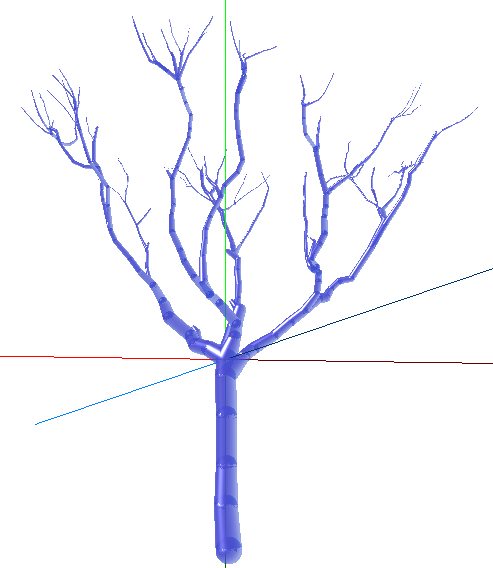
\includegraphics[height=6cm]{uc6_1.png}}\hspace{5em}
	\subfloat[纵向简化(后)]{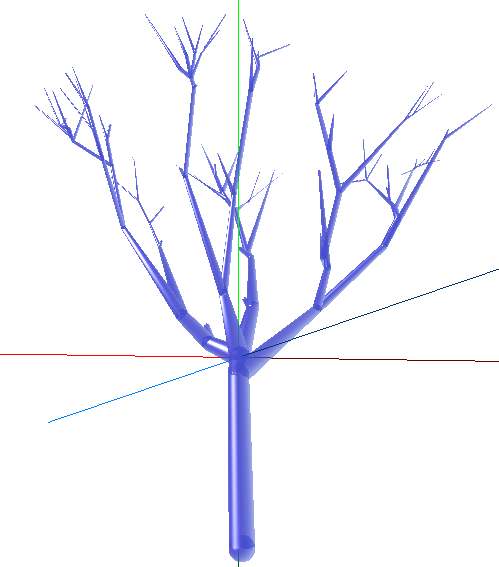
\includegraphics[height=6cm]{uc6_2.png}}\hspace{5em}
	\caption{用例图示:简化模型}
	\label{fig:uc6}
\end{figure}

\begin{table}[H]
	\centering
\begin{tabular}{|l|p{8cm}|}
	\hline
	用例名称: & 简化模型\\
	\hline
	用例标志号: & 6\\
	\hline
	参与者: & 用户\\
	\hline
	简要说明: & 用户可以通过选择某棵子树,对其进行如第\ref{cha:branchcombine}章中的合并操作,以简化模型。具体效果见图\ref{fig:uc6}\\
	\hline
	前置条件: & 树木的显示模式为骨架模型\\
	\hline
	基本事件流: & 1. 用户按下's'键\\
	 & 2. 对当前节点及其表示的子树进行基于合并的简化\\
	 & 3. 用例终止\\
	\hline
	后置条件: & 无\\
	\hline
\end{tabular}
\end{table}

\clearpage
\section{泛洪算法演示}
\begin{figure}[H]
	\centering
	\subfloat[输入:从点云中得到的体素模型]{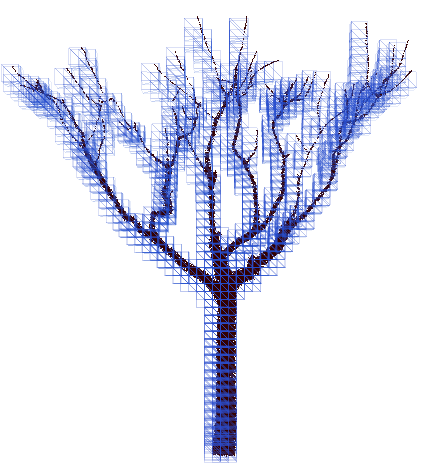
\includegraphics[width=0.35\linewidth]{uc7_1.png}}\hfill
	\subfloat[泛洪算法初始化]{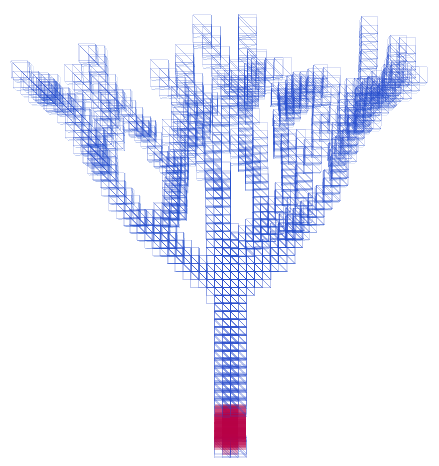
\includegraphics[width=0.35\linewidth]{uc7_2.png}}\hfill
	\subfloat[泛洪算法中间步骤]{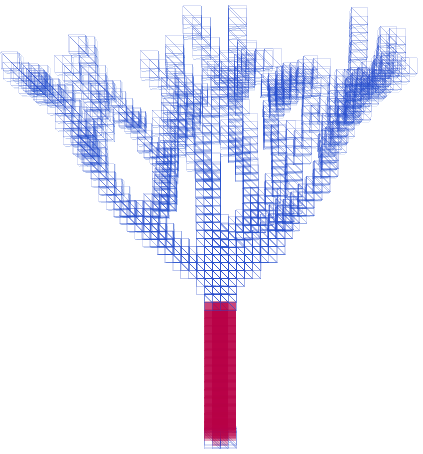
\includegraphics[width=0.35\linewidth]{uc7_3.png}}\hfill
	\subfloat[泛洪算法完成]{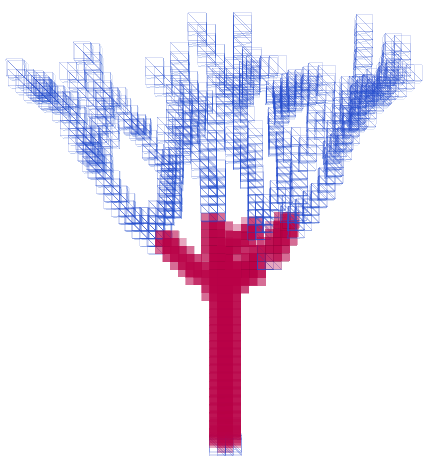
\includegraphics[width=0.35\linewidth]{uc7_4.png}}
	\caption{用例图示:泛洪算法演示}
	\label{fig:uc7}
\end{figure}

\begin{table}[H]
	\centering
\begin{tabular}{|l|p{8cm}|}
	\hline
	用例名称: & 泛洪算法演示\\
	\hline
	用例标志号: & 7\\
	\hline
	参与者: & 用户\\
	\hline
	简要说明: & 用户可以根据输入的点云,进行泛洪算法的可视化单步观察。具体效果见图\ref{fig:uc7}\\
	\hline
	前置条件: & 树木的点云数据已经被加载进入程序,并且打开了体素模型模式\\
	\hline
	基本事件流: & 1. 用户按下'e'键\\
	 & 2. 对当前节点进行泛洪并找到其字节点\\
	 & 3. 选中其子节点,并重复1和2中的步骤\\
	 & 4. 当达到叶子节点时,用例结束\\
	\hline
	后置条件: & 无\\
	\hline
\end{tabular}
\end{table}

